\documentclass[aspectratio=169]{beamer}

\mode<presentation>
{
  \usetheme{default}
  \usecolortheme{seahorse}
  \usefonttheme{professionalfonts}
  \setbeamertemplate{navigation symbols}{}
  \setbeamertemplate{caption}[numbered]
  \setbeamertemplate{footline}[frame number]
}

\usepackage[utf8x]{inputenc}
\usepackage{graphicx}
\usepackage{physics}
\usepackage{caption}
\usepackage{subcaption}
\usepackage{xcolor}
\usepackage{physics}
\usepackage{amsmath}
\usepackage{tikz}
\usepackage{mathdots}
\usepackage{yhmath}
\usepackage{cancel}
\usepackage{color}
\usepackage{siunitx}
\usepackage{array}
\usepackage{multirow}
\usepackage{amssymb}
\usepackage{gensymb}
\usepackage{tabularx}
\usepackage{extarrows}
\usepackage{booktabs}
\usetikzlibrary{fadings}
\usetikzlibrary{patterns}
\usetikzlibrary{shadows.blur}
\usetikzlibrary{shapes}



\title[quali_slides]{Online tuning of storage ring non-linear dynamics at SIRIUS and fast ORM measurement}

\author{Matheus Melo Santos Velloso \\{\small Ms.C student}\\
\vspace{0.5cm}
on behalf of the LNLS Accelerator Physics Group}

\institute{Gleb Wataghin Institute of Physics - University of Campinas\\ Accelerator Physics Group (FAC) -  Brazilian Syncrhotron Laboratory (LNLS)}

\date{June 2023}

\AtBeginSection[]
{
    \begin{frame}
         \tableofcontents[currentsection]
   \end{frame}
}

\begin{document}
\maketitle
\begin{frame}{Contents}
    \tableofcontents
\end{frame}

\section{Introduction}
\begin{frame}{SIRIUS}
    \begin{minipage}{0.45\textwidth}
        \begin{figure}
            \centering
            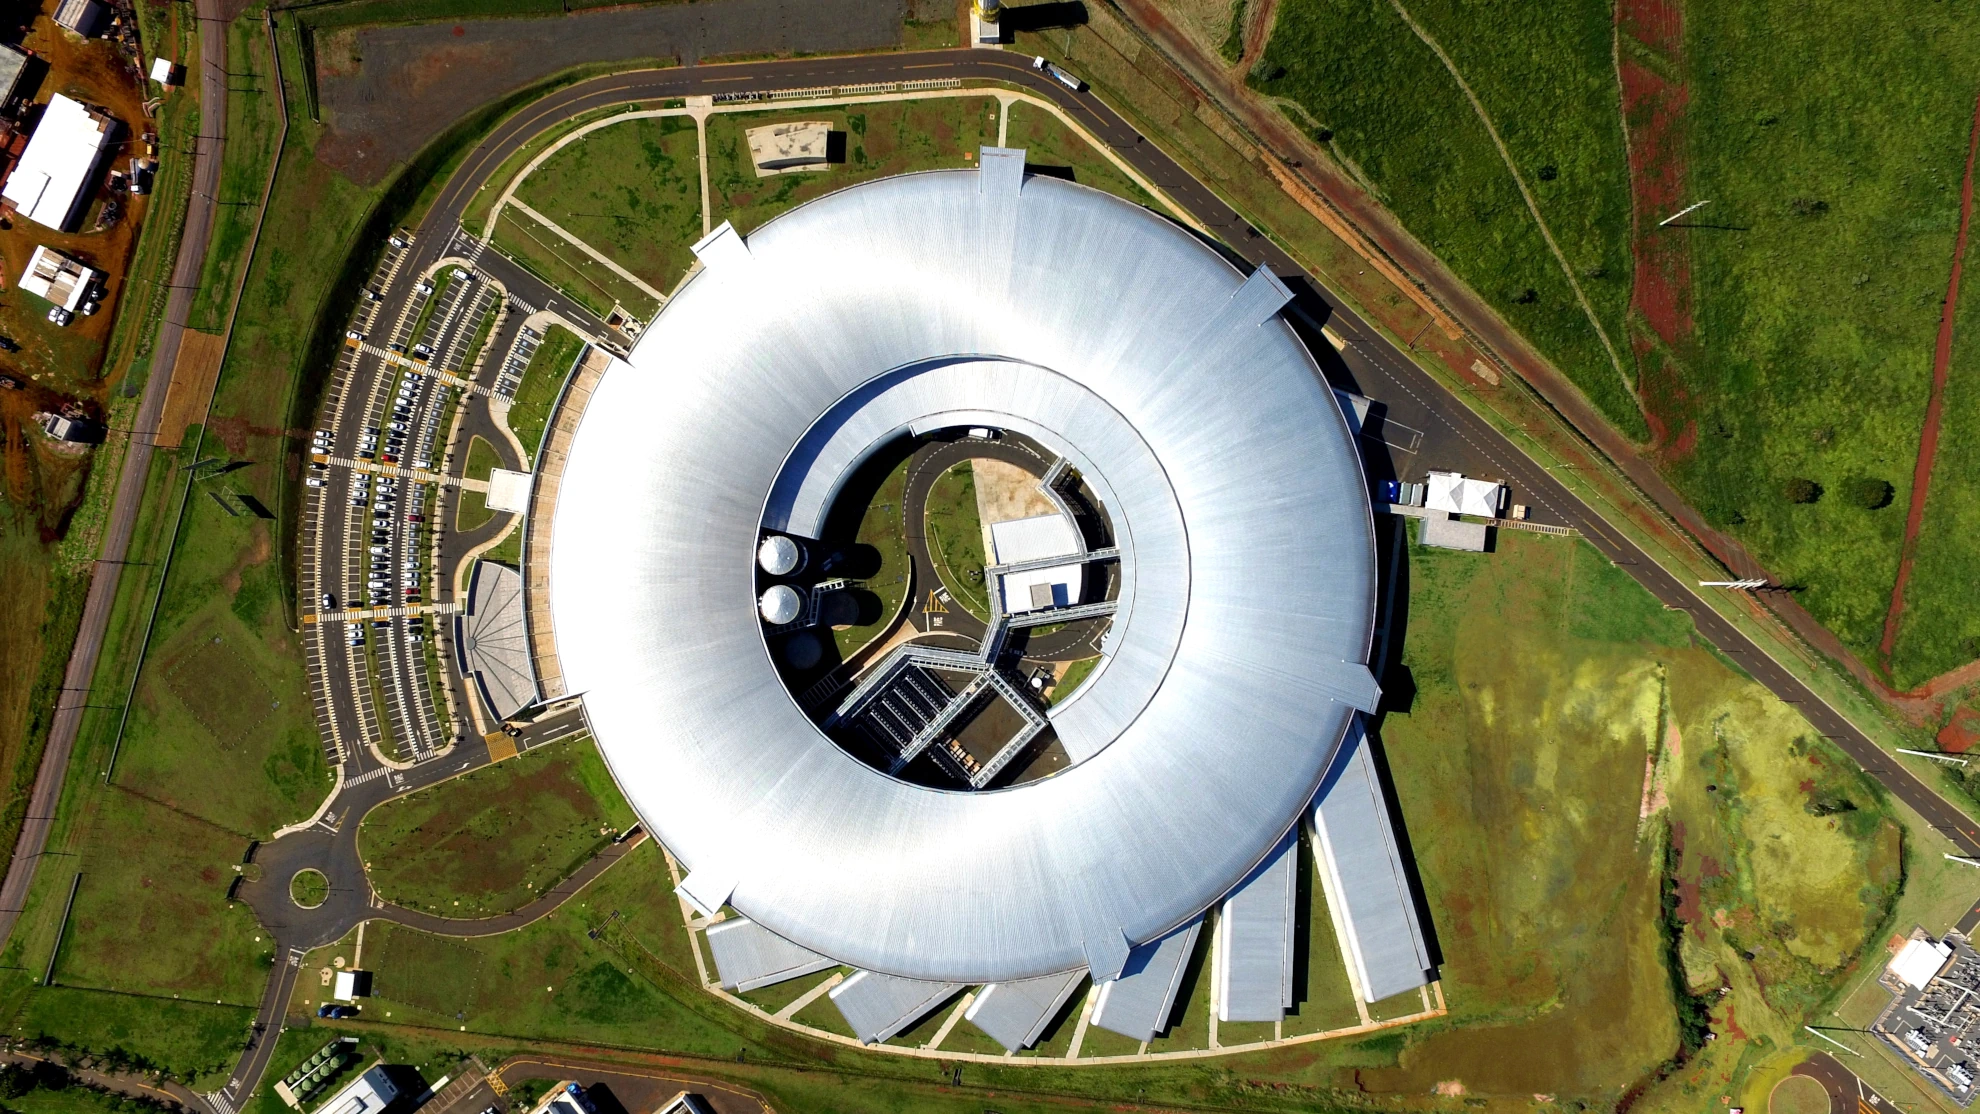
\includegraphics[width=\textwidth]{f1.png}
        \end{figure}
    \end{minipage}
    \hfill
    \begin{minipage}{0.45\textwidth}
        \begin{itemize}
            \item 4th generation storage ring-based synchrotron light source
            \item LINAC, booster, storage ring
            \item Storage ring: $518~\unit{\m}$ in circumf, $3~\unit{GeV}$, nominal energy
            \item $100~\unit{mA}$ current, top-up injection mode
        \end{itemize}
    \end{minipage}
\end{frame}

\begin{frame}{The dissertation problem}
    Off-axis injection scheme
    \begin{figure}
        \centering
        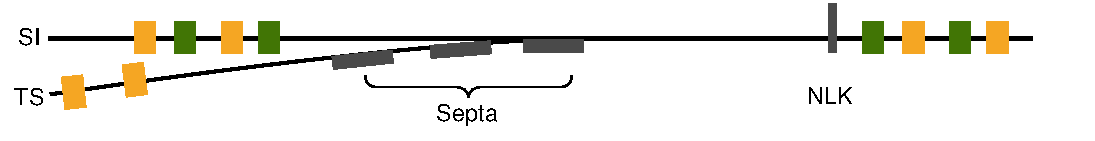
\includegraphics[width=0.7\textwidth]{injection.pdf}
    \end{figure}
    \pause
    \begin{figure}
        \centering
        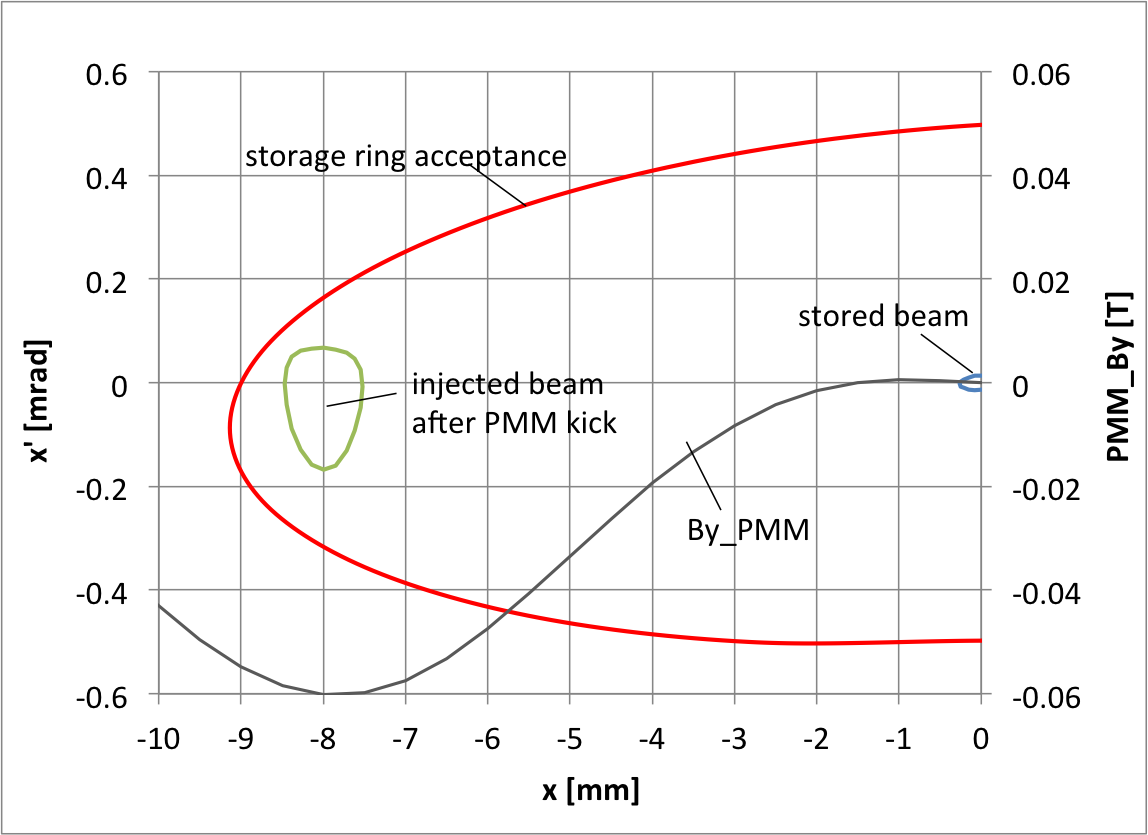
\includegraphics[width=0.6\textwidth]{nlk_phase_space.png}
    \end{figure}
\end{frame}

\section{Online optimization of Dynamic Aperture}
\begin{frame}{SIRIUS Dynamic Aperture Optimization}
    \begin{minipage}{0.55\textwidth}
        Working point $\nu_x, = 49.08, \nu_y = 14.14$
        \begin{figure}
            \centering
            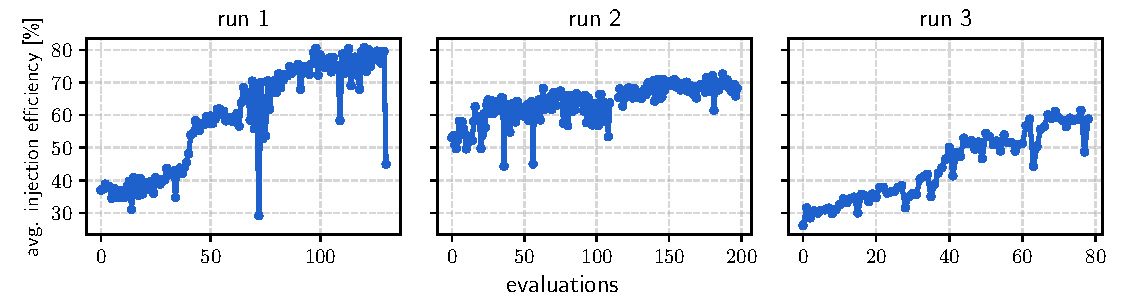
\includegraphics[width=\textwidth]{oldtunes_history.pdf}
            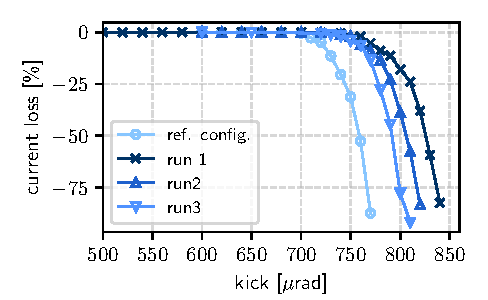
\includegraphics[width = 0.8\textwidth]{WEPL087_f1.pdf}
            \vfill
            \begin{itemize}
                \item injection efficiency: $98\pm1~\%$ run 2
                \item 1 hour reduction in lifetime
            \end{itemize}
        \end{figure}
    \end{minipage}
    \hfill
    \begin{minipage}{0.44\textwidth}
        \begin{figure}
            \centering
            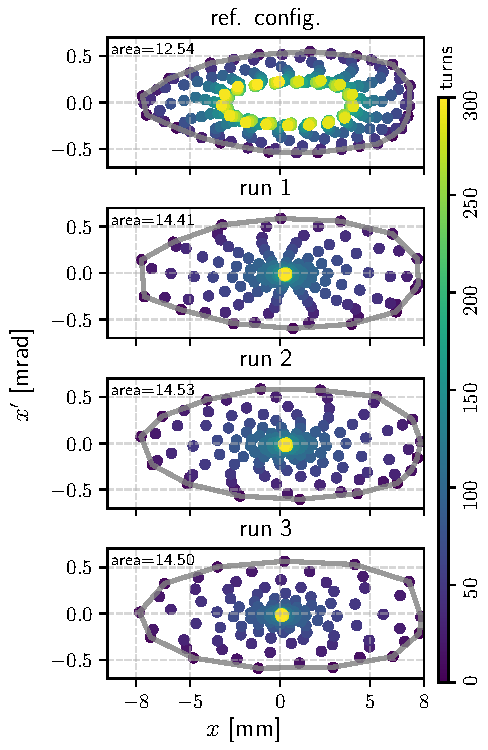
\includegraphics[height=0.9\textheight]{WEPL087_f2.pdf}
        \end{figure}
    \end{minipage}
\end{frame}
\begin{frame}{SIRIUS Dynamic Aperture Optimization}
    \begin{minipage}{0.55\textwidth}
        Working point $\nu_x, = 49.20, \nu_y = 14.25$
        \begin{figure}
            \centering
            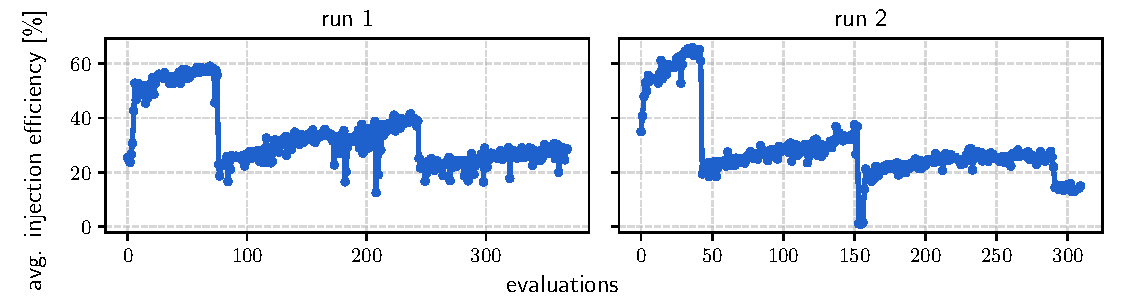
\includegraphics[width=\textwidth]{newtunes_history.pdf}
            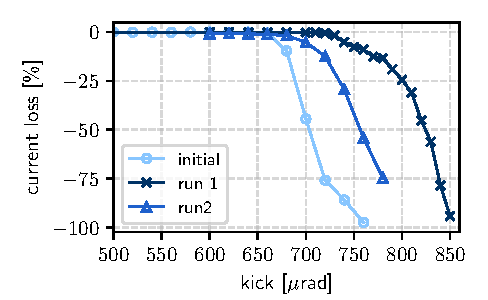
\includegraphics[width = 0.8\textwidth]{WEPL087_f3.pdf}
            \begin{itemize}
                \item injection efficiency: $79\pm3~\%$ run 1
                \item no reduction in lifetime
            \end{itemize}
        \end{figure}
    \end{minipage}
    \hfill
    \begin{minipage}{0.44\textwidth}
        \begin{figure}
            \centering
            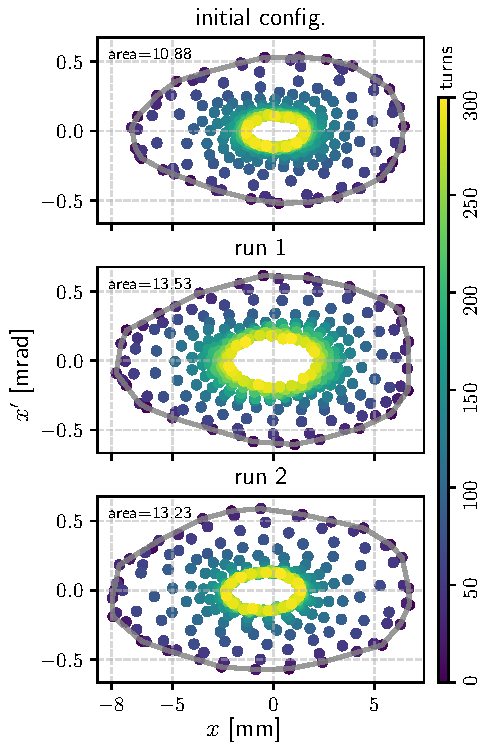
\includegraphics[height=0.9\textheight]{WEPL087_f4.pdf}
        \end{figure}
    \end{minipage}
\end{frame}
\begin{frame}{SIRIUS Dynamic Aperture Optimization}
    \begin{minipage}{0.55\textwidth}
        Working point $\nu_x, = 49.16, \nu_y = 14.22$
        \begin{figure}
            \centering
            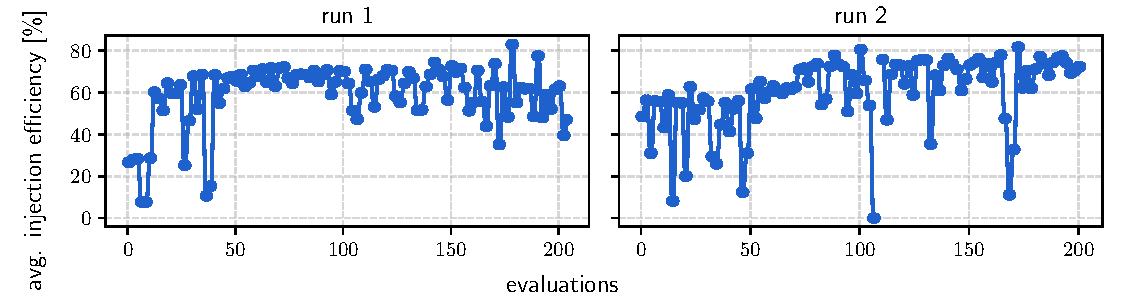
\includegraphics[width=\textwidth]{wp3_history.pdf}
            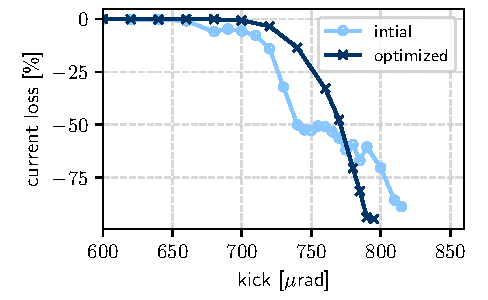
\includegraphics[width = 0.8\textwidth]{wp3_kick_resilience.pdf}
            \begin{itemize}
                \item injection efficiency: $93\pm3~\%$ run 1
                \item 1.5 hr reduction in lifetime
            \end{itemize}
        \end{figure}
    \end{minipage}
    \hfill
    \begin{minipage}{0.44\textwidth}
        \begin{figure}
            \centering
            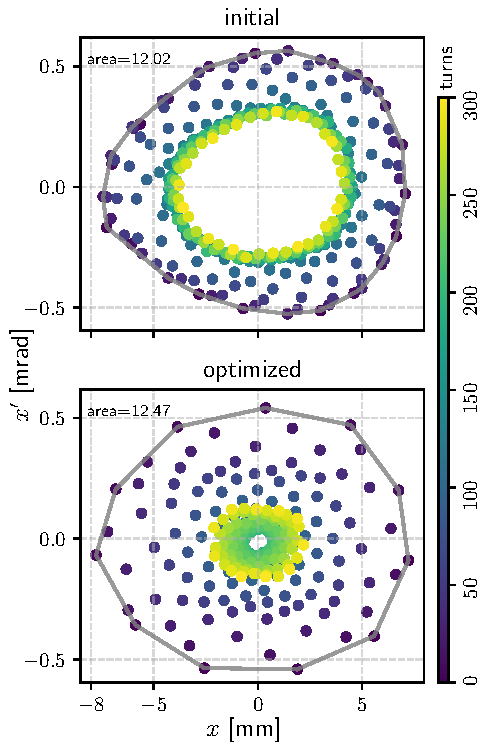
\includegraphics[height=0.9\textheight]{wp3_phase_space.pdf}
        \end{figure}
    \end{minipage}
\end{frame}
\begin{frame}
    Thank you!
\end{frame}

\section{Fast ORM Measruement}
\end{document}
